\section{Robustness}
\label{sec:robustness}

This section reports the disciplining battery: the PIT correction that bounds the population scope of the result, the functional-form sensitivity of the quadratic-IO clearance, the pre/post-2015 temporal split, the instrumental-variables strategy that fails its first-stage relevance test, the within-retail aggregation-artifact null, the variance-channel diagnostic, and the inference discipline.

\subsection{The PIT correction and the nested-baseline collapse}
\label{sec:robust_pit}

The seed prior to this paper's revisions predicted a negative aggregate three-way on the full panel and a negative within-stock retail-versus-institutional difference. Table~\ref{tab:nested} reports both objects under the static-snapshot literacy merge and under the point-in-time EDGAR 10-K-header literacy reassignment.

\begin{table}[t]
\centering
\caption{The nested baseline: aggregate and mid-IO three-way under PIT correction}
\label{tab:nested}
\footnotesize
\begin{minipage}{\textwidth}
\centering
\textit{Panel A: Aggregate three-way coefficient}\\[2pt]
\begin{tabular}{lrrrr}
\toprule
Specification & $\hat\gamma$ & State-$t$ & wcb $p$ & $N$ \\
\midrule
Full panel, static-snapshot literacy & $-0.0117$ & $-2.17$ & 0.078 & 623,896 \\
Full panel, PIT literacy reassignment & $-0.0003$ & $-0.86$ & 0.517 & 623,814 \\
Stable-HQ subsample, static literacy  & $-0.0145$ & $-1.94$ & 0.122 & 519,090 \\
\bottomrule
\end{tabular}

\medskip
\textit{Panel B: Mid-IO coefficient under PIT, with and without size controls}\\[2pt]
\begin{tabular}{lrrrr}
\toprule
Specification & $\hat\gamma_{\text{mid-IO}}$ & State-$t$ & Collapse vs.\ baseline & $N$ \\
\midrule
Stable-HQ static, persistent (paper headline) & $-0.0321$ & $-2.63$ & --- & 191,589 \\
Stable-HQ static, size-controlled & $-0.0256$ & $-2.24$ & --- & 191,589 \\
PIT full panel, persistent & $-0.00121$ & $-2.07$ & $\approx 27\times$ smaller & 191,589 \\
PIT full panel, size-controlled & $-0.00100$ & $-1.75$ & $\approx 26\times$ smaller & 191,589 \\
\bottomrule
\end{tabular}
\end{minipage}

\medskip
{\footnotesize\textit{Notes.} Static-snapshot merge pairs each firm-month with the literacy of its Compustat \texttt{state}; PIT reassignment re-merges against the firm's then-current 10-K-header state and re-$z$-scores within month. State-level wild-cluster bootstrap (Webb six-point, $B = 4{,}999$ or $9{,}999$, null imposed). The PIT magnitude collapse is essentially the same with and without size controls (27$\times$ vs.\ 26$\times$).}
\end{table}

Two readings of the PIT magnitude collapse compete on the discriminating margins this design supports. A \textit{mechanism-strength reading} says the mechanism operates most strongly on stable-HQ firms (where the local-investor unit of analysis is well-defined); the corrected full panel including the 14\% of firm-months with relocated headquarters dilutes the average. A \textit{sample-selection reading} says the stable-HQ subsample is sample-selected toward firms with stronger anomaly moderation for reasons orthogonal to the literacy channel; the 26$\times$ ratio is therefore an artifact of which firms remain in the sample. The relocator characteristics in IA~\ref{ia:relocchar} --- relocators are smaller, higher-IV, lower-IO, lower-return firms --- lean toward the sample-selection reading. The mechanism-strength reading is not defendable on current evidence. The paper's interaction-zone characterization is a statement about the stable-HQ population; generalization to the PIT-corrected full panel is the principal population-scope limitation.

\subsection{Functional-form grid for the quadratic-IO U-shape}
\label{sec:robust_form}

The continuous-margin quadratic-IO five-percent clearance ($\hat\gamma_{5} = +0.0151$, $p = 0.017$) does not survive alternative functional forms. Table~\ref{tab:form_grid} reports the grid.

\begin{table}[t]
\centering
\caption{Functional-form grid: the quadratic five-percent clearance is parametric}
\label{tab:form_grid}
\footnotesize
\begin{minipage}{\textwidth}
\centering
\begin{tabular}{lcccr}
\toprule
Specification & Focal term & Coef & State-$t$ & wcb $p$ \\
\midrule
\textbf{Quadratic (corroborating)} & $\gamma$ on IO$^{2}$ & $\mathbf{+0.0151}$ & $\mathbf{+2.28}$ & $\mathbf{0.017}$ \\
Cubic & $\gamma$ on IO$^{3}$ & $+0.798$ & $+1.70$ & 0.133 \\
Log-IO & $\gamma$ on $\log(\mathrm{IO})$ & $-0.00243$ & $-0.35$ & 0.748 \\
Kink-IO at 0.30 & kink coef & $+0.179$ & $+1.19$ & 0.242 \\
20-bin diagnostic & conditional means within $\pm 0.003$ of zero & --- & --- & --- \\
\bottomrule
\end{tabular}
\end{minipage}

\medskip
{\footnotesize\textit{Notes.} Stable-HQ persistent-IO subsample. Each row reports the focal-basis coefficient with state-clustered $t$ and wild-cluster bootstrap $p$. The 20-bin diagnostic partitions persistent IO into 20 quantile bins, residualizes the focal triple's contribution to monthly returns on state and month fixed effects within each bin, and reports the within-bin conditional mean of the demeaned composite.}
\end{table}

Log-IO returns a coefficient near zero ($p = 0.75$). Kink-IO at the empirical minimum delivers neither a kink coefficient nor a linear term separable from zero. The 20-bin diagnostic shows bin-level conditional means within $\pm 0.003$ of zero across the IO range, with no visible monotonic curvature. The 5-percent statistical clearance of the U-shape rests on the quadratic functional form alone; the discrete-tercile mid-IO concentration (Table~\ref{tab:headline}) is functional-form-free and remains the load-bearing characterization.

\subsection{Pre/post-2015 split and time variation}
\label{sec:robust_prepost}

The within-panel mid-IO three-way coefficient is essentially identical pre- and post-2015 ($\hat\gamma^{\text{pre}} = -0.024$, $t = -1.27$; $\hat\gamma^{\text{post}} = -0.026$, $t = -1.14$; difference $-0.002$, $t = +0.06$). The within-panel direction is stable across the sample. What changes across time is the cross-state literacy gradient that interprets the result through the literacy mechanism. Table~\ref{tab:prepost_grad} reports the gradient by sub-period.

\begin{table}[t]
\centering
\caption{Cross-state literacy gradient by sub-period (size-controlled, mid-IO)}
\label{tab:prepost_grad}
\footnotesize
\begin{minipage}{\textwidth}
\centering
\begin{tabular}{lcccc}
\toprule
Period & Weighted slope & state-$t$ & Pearson $r$ & $n_{\text{states}}$ \\
\midrule
Pre-2015 (2009--2014) & $+0.0403$ & $+1.89$ & $+0.048$ & 37 \\
Post-2015 (2015--2023) & $\mathbf{-0.0706}$ & $\mathbf{-3.50}$ & $-0.370$ & 38 \\
Pooled (2009--2023) & $\mathbf{-0.0623}$ & $\mathbf{-5.01}$ & $-0.275$ & 42 \\
\midrule
NFCS Wave 2009 only (2009--2011) & $+0.281$ & $+2.57$ & $+0.109$ & 34 \\
NFCS Waves 2012--2021 & $-0.114$ & $-1.18$ & $-0.066$ & --- \\
\bottomrule
\end{tabular}
\end{minipage}

\medskip
{\footnotesize\textit{Notes.} Per-state $\hat\gamma_{\text{lit}}$ from Equation~\eqref{eq:size_ctrl} with month fixed effects only; precision-weighted cross-state regression. States with $\geq 5$ firms in the sample cell. Wave-2009 row segregates the first NFCS administration (which produced the wrong-signed cross-state gradient driving the entire pre-2015 result).}
\end{table}

Figure~\ref{fig:time} visualizes the time variation. Panel A shows the rolling 5-year-window mid-IO three-way coefficient is negative in every window. Panel B shows the pre/post-2015 cross-state gradient: all pre-2015 cells are positive (wrong sign), all post-2015 mid-IO and high-IO cells are negative (right sign). Panel C reports the size-filter migration heatmap by sub-period.

\begin{figure}[t]
\centering
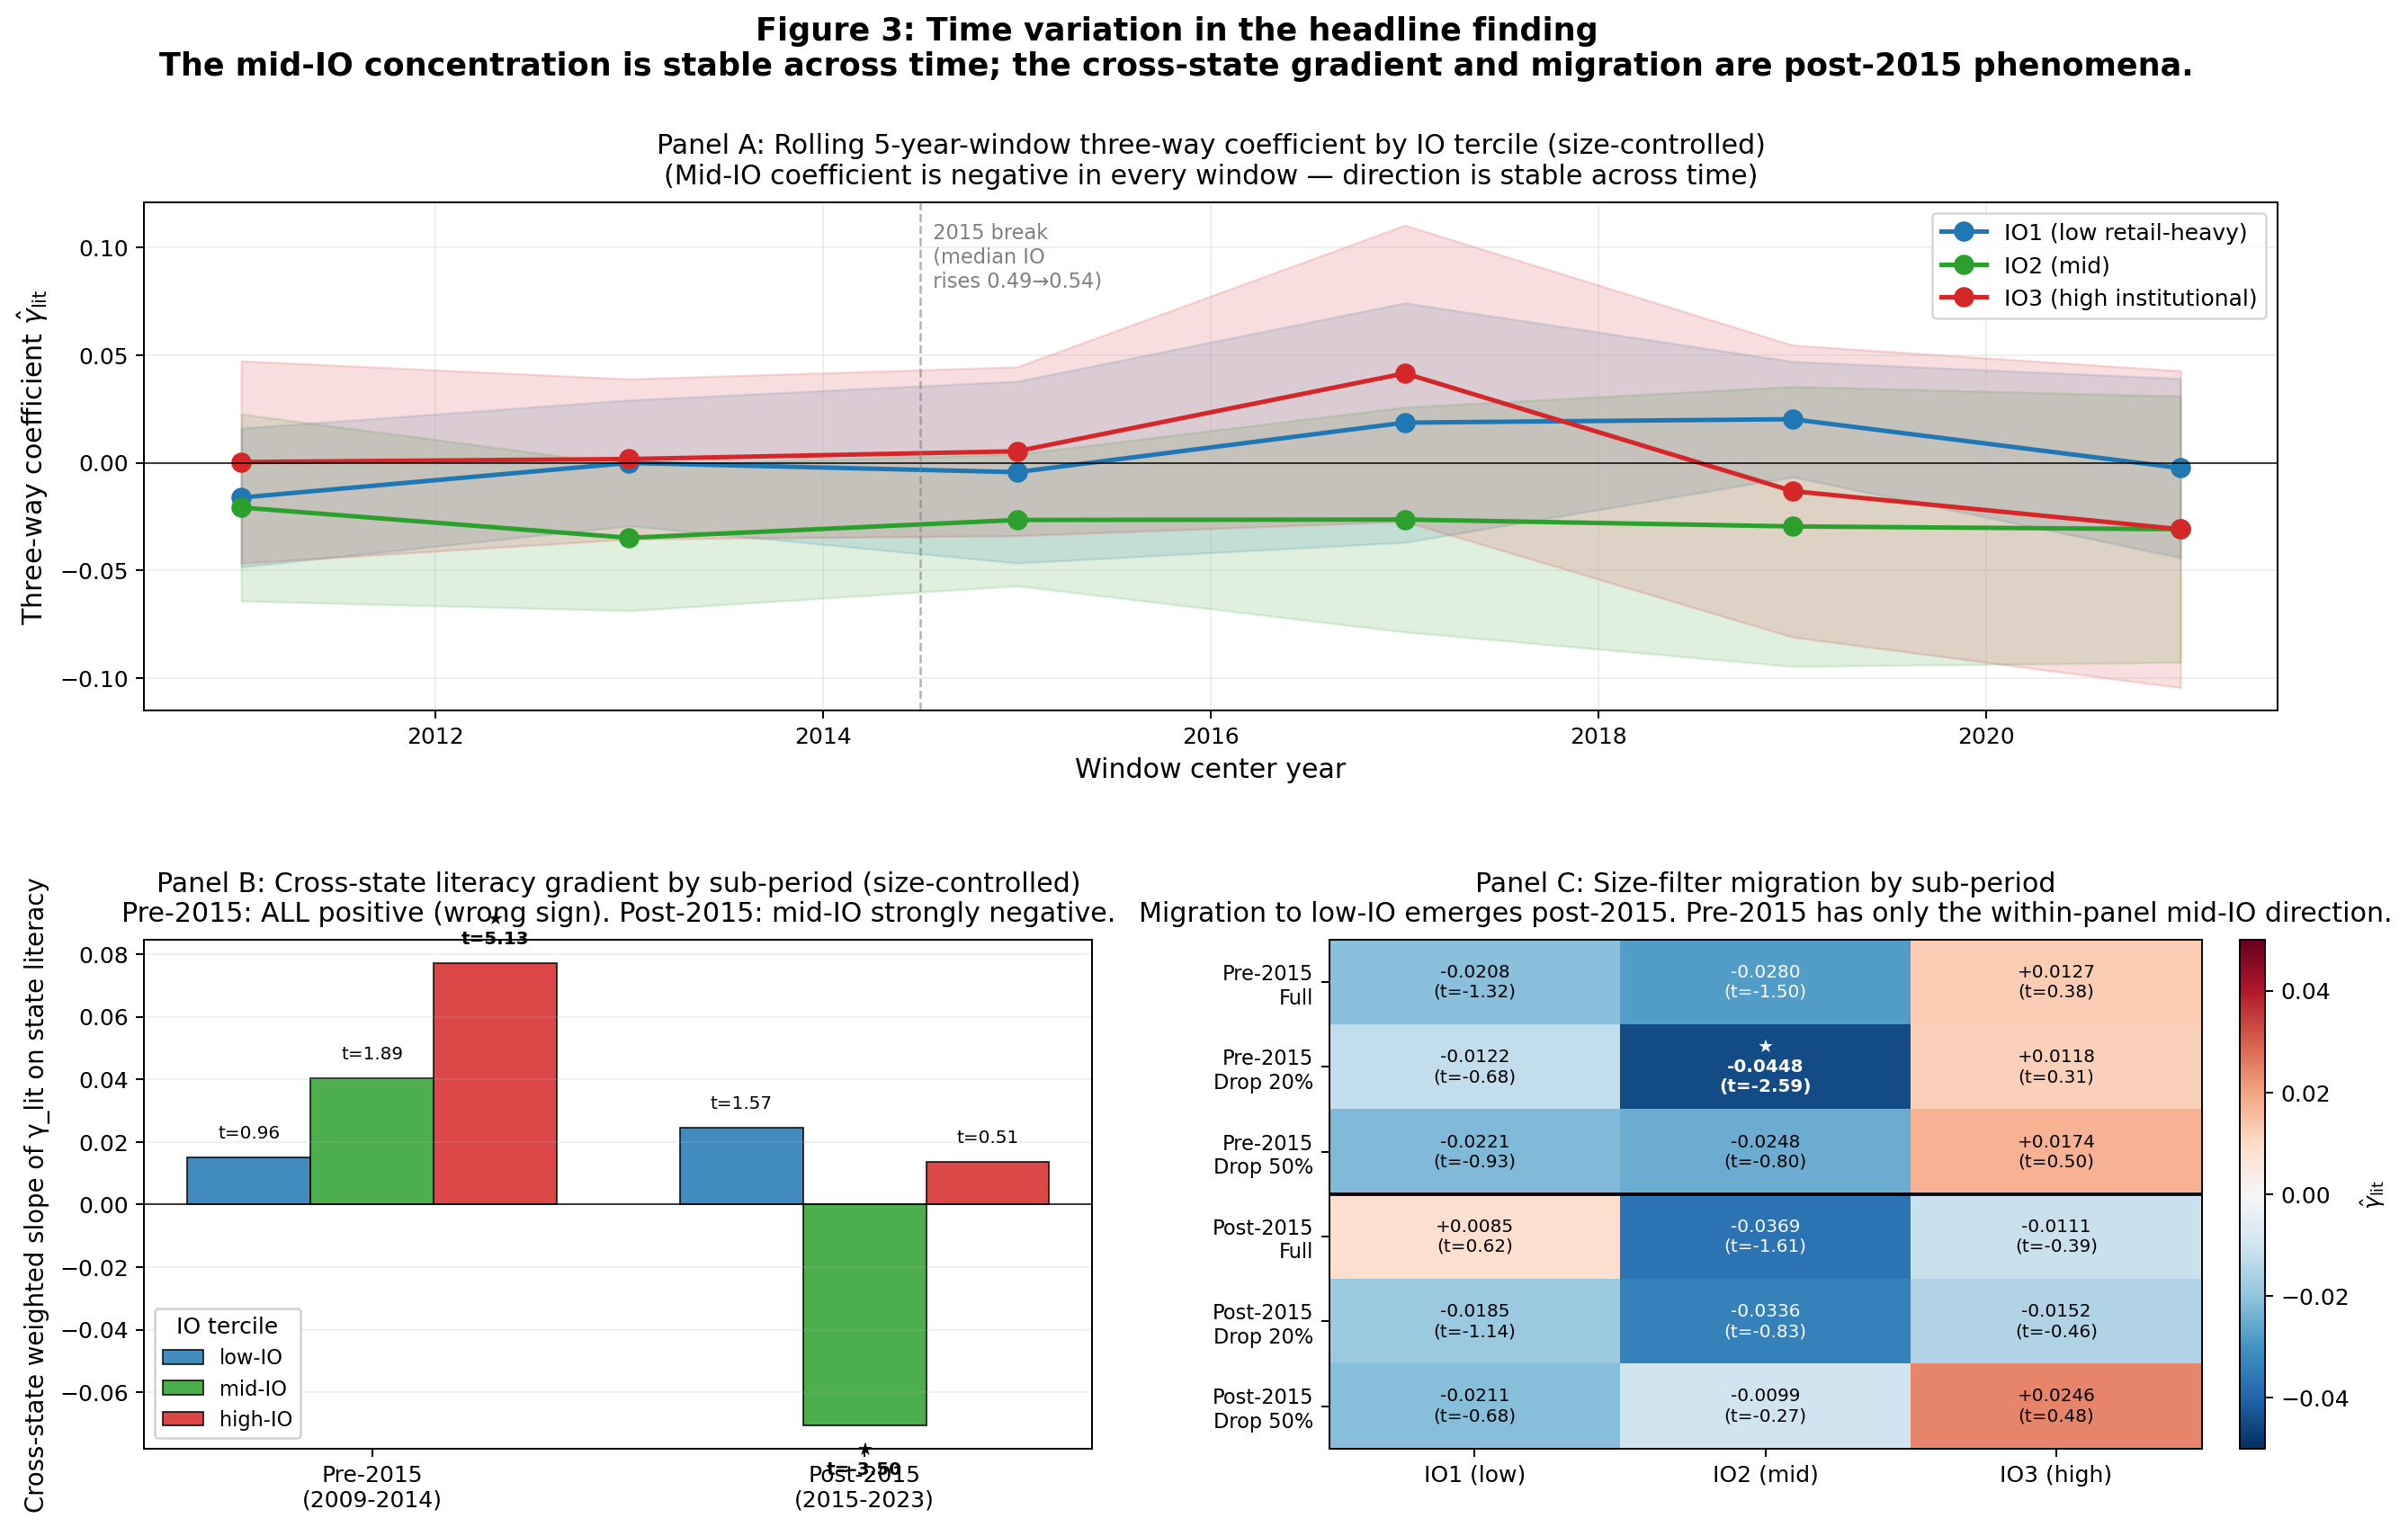
\includegraphics[width=\textwidth]{figures/figure3_time.png}
\caption{Time variation in the headline finding. Panel A: rolling 5-year-window mid-IO three-way coefficient is negative in every window. Panel B: cross-state literacy gradient by sub-period --- pre-2015 cells are wrong-signed, post-2015 cells are right-signed. Panel C: size-filter migration heatmap by sub-period.}
\label{fig:time}
\end{figure}

The pre-2015 cross-state slope is wrong-signed ($+0.040$, $t = +1.89$); the post-2015 slope is right-signed and significant ($-0.071$, $t = -3.50$); the pooled slope is in between and benefits from doubled sample size ($-0.062$, $t = -5.01$). The wrong-signed pre-2015 result is concentrated in NFCS Wave 2009 (slope $+0.281$, $t = +2.57$), the first administration of the Big-Five module; Waves 2012--2021 are directionally negative.

The most parsimonious explanation is NFCS measurement maturation in the 2015+ waves rather than a 2015-era economic regime change. Institutional ownership of the panel firms \textit{rose} post-2015 (mean change $+0.083$ in $\mathtt{io\_share}$ pre-to-post), not fell, ruling out the retail-trading regime hypothesis (Robinhood March 2015, commission-free industry adoption October 2019) as the mechanism for the strengthening cross-state gradient. The state-level change in IO does not correlate with state literacy (Pearson $r = +0.04$, $p = 0.80$). The 2009 NFCS wave is the unique outlier; the cross-state gradient appears in the data once it is excluded.

\subsection{Instrumental-variables strategy: documented first-stage failure}
\label{sec:robust_iv}

I attempted to instrument state $\mathtt{literacy\_z}$ with state-level exposure to K-12 personal-finance graduation requirements, using the Urban-Schmeiser 2015 database as updated through Burke-Collins-Urban (2023). The instrument fails its first-stage relevance test in the relevant direction.

\paragraph{Cross-state first stage.}

\begin{table}[t]
\centering
\caption{First-stage diagnostics: NFCS state literacy on mandate exposure}
\label{tab:fs_iv}
\footnotesize
\begin{minipage}{\textwidth}
\centering
\begin{tabular}{lccc}
\toprule
Instrument & Slope & Pearson $r$ & First-stage $F$ \\
\midrule
has\_pf\_mandate (ever-treated by 2024) & $-1.31$ & $\mathbf{-0.355}$ & $\mathbf{7.06}$ \\
early\_pf\_adopter (treated by 2000) & $+0.72$ & $+0.112$ & 0.62 \\
cohort\_share\_affected & $-0.59$ & $-0.051$ & 0.13 \\
log\_years\_pf & $-0.27$ & $-0.171$ & 1.47 \\
\bottomrule
\end{tabular}
\end{minipage}

\medskip
{\footnotesize\textit{Notes.} Cross-state regression of state NFCS literacy (panel mean \%) on each candidate instrument, $n = 51$ states. The strongest candidate (has\_pf\_mandate) has $r = -0.355$ (wrong sign for a positive IV) and $F = 7.06$ (below the Stock-Yogo $F > 10$ threshold). The mandate-literacy correlation is negative because the South and Appalachia (low-literacy regions) adopted mandates as a remedy; the Northeast and Pacific (high-literacy regions) did not. This is reverse causality, not a flaw in the underlying literacy story.}
\end{table}

\paragraph{Cohort-matched first stage.} The right way to instrument adult literacy with K-12 mandates is to match the mandate window to the affected cohort. NFCS includes age band $\mathtt{A3Ar\_w}$ (six bands: 18--24, 25--34, 35--44, 45--54, 55--64, 65+) in every wave; I constructed a state $\times$ wave $\times$ age-band panel (1{,}530 cells) and computed cohort-specific mandate exposure as the fraction of each band's HS-graduation years that overlap the state's mandate window. The first-stage regresses pass-3 literacy on cohort exposure with progressive fixed effects. Without controls the slope is $-0.106$, $t = -12.9$ --- driven by the obvious confound that younger respondents have both lower literacy and higher cohort exposure. With State + Wave + Band fixed effects, which compare like-aged respondents across states and waves, the slope becomes $+0.002$, $t = +0.22$, partial $F = 0.05$. The cohort-matched instrument is no stronger than the aggregate instrument under the right controls.

\paragraph{2SLS results.} Running 2SLS anyway in the mid-IO size-controlled spec returns standard errors inflated 6--7$\times$ relative to OLS, with all $t$-statistics below 2: $\hat\gamma_{2SLS} = -0.062$ ($t = -0.83$) under share-affected instrument; $\hat\gamma_{2SLS} = -0.071$ ($t = -1.08$) under log-years instrument; $\hat\gamma_{2SLS} = -0.016$ ($t = -0.21$) under has-mandate instrument. Direction is right; precision is destroyed. The OLS estimate $\hat\gamma_{\text{OLS}} = -0.0256$ ($t = -2.24$) remains the preferred inferential statement.

\paragraph{Why the IV fails.} Three forces combine. State mandates are too recent: most adoptions are 2005--2014, so substantial exposure is concentrated in the 18--24 age band only. School-level compliance with state mandates is only $\approx 48\%$ \citep{urban2020}, halving the intent-to-treat exposure. The NFCS Big-Five instrument is a narrow five-question test (interest compounding, inflation, diversification, mortgages, bond pricing); mandate-affected cohorts may have higher \textit{broad} financial knowledge but not higher Big-Five scores specifically. The IV strategy is left for future work that can exploit cohort-specific NFCS micro-data on a broader literacy measure.

\subsection{Within-retail wrong-sign null and IV-decile decomposition}
\label{sec:robust_withinretail}

Within the stable-HQ low-IO tercile, splitting at the within-tercile state-mean literacy median delivers a low-literacy-minus-high-literacy difference in the three-way of $+0.0033$ persistent (state-clustered $t = +2.80$, wild-cluster bootstrap $p = 0.024$). The sign is wrong from the naive sophistication reading. A within-month NYSE IV-decile decomposition shows the difference is an aggregation artifact: five deciles return positive differences and five return negative, only decile 8 is individually significant, and the observation-weighted average is $+0.0002$. The aggregate $+0.0033$ is entirely attributable to observation-weighting and decomposes to approximately zero across IV deciles. The sign reversal provides no positive evidence against the naive sophistication reading and does not separate within-family candidates. Detail is in IA~\ref{ia:ivdecile}.

\subsection{Variance-channel diagnostic and college horse-race}
\label{sec:robust_variance}

A purely statistical reading would attribute the mid-IO concentration to greater identifying variation at the mid tercile. Within-tercile variances of the focal triple $\mathrm{mom}\cdot\mathrm{IV}\cdot\mathtt{literacy\_z}$ on the stable-HQ subsample are $1.664$ (low-IO), $0.673$ (mid-IO), and $0.434$ (high-IO); Bartlett's equal-variance test rejects strongly, and the same ordering survives state-month demeaning. Mid-IO has lower identifying variation than low-IO yet a larger slope, so the variance channel cannot explain the mid-vs-low contrast. The mid-vs-high ranking is consistent with the variance ordering and is not the discriminating margin.

The state college-attainment horse-race within mid-IO returns $\hat\gamma_{\text{lit}} = -0.0350$ ($t = -2.97$) and $\hat\gamma_{\text{college}} = +0.00076$ ($t = +0.65$): the literacy three-way sharpens relative to the literacy-only mid-IO baseline of $-0.0321$, and the college three-way is opposite-signed and indistinguishable from zero. Literacy is not a proxy for college attainment within mid-IO.

\subsection{Inference discipline}
\label{sec:robust_inference}

One-way state clustering on the literacy three-way is the binding inference dimension: 51 state clusters are the natural support of the focal variable. The state-level wild-cluster bootstrap of \citet{cameronGelbachMiller2008} with Webb six-point weights \citep{webb2014} and the null imposed is the appropriate small-cluster procedure. For the cross-state literacy gradient, the precision-weighted-slope $t$-statistic is interpreted alongside a state-permutation $p$-value with $B = 9{,}999$. The Holm step-down family-wise correction across the three-test family (T1, T2, T3 in Section~\ref{sec:cross_state_grad}) is the FWER-controlled multiplicity adjustment; Romano-Wolf step-down with joint resampling would be no larger than the Holm bound and is therefore a conservative upper bound on the FWER $p$-value.

\subsection{Wave-anchor and 2009-vintage forward-fill}
\label{sec:robust_vintage}

Restricting to the five NFCS wave-anchor years only (2009, 2012, 2015, 2018, 2021; $N = 174{,}226$ firm-months, 62{,}032 in mid-IO), the persistent mid-IO three-way is $\hat\gamma_{\text{mid}} = -0.070$ ($t = -2.09$): sharper, not weaker, than the interpolated monthly headline. The headline is not an artifact of forward-fill. Fixing each firm's IO tercile to its 2009 full-year-mean IO assignment (only $\approx 5\%$ of firms drift under the persistent IO measure) attenuates the mid/low ratio from $2.83$ to $2.09$ but preserves the mid-IO concentration. The secular-IO-shift reading of the concentration is bounded.
